%%
%% Copyright 2007, 2008, 2009 Elsevier Ltd
%%
%% This file is part of the 'Elsarticle Bundle'.
%% ---------------------------------------------
%%
%%
\documentclass[preprint,3p,10pt,twocolumn,number,sort&compress]{elsarticle}
%\documentclass[final,3p,10pt,twocolumn,number,sort&compress]{elsarticle}

%\usepackage{lipsum}
%\makeatletter
%\def\ps@pprintTitle{%
 %\let\@oddhead\@empty
 %\let\@evenhead\@empty
% \def\@oddfoot{}%
% \let\@evenfoot\@oddfoot}
%\makeatother
%\documentclass[preprint,12pt]{elsarticle}

%% Use the option review to obtain double line spacing
%% \documentclass[preprint,review,12pt]{elsarticle}

%% Use the options 1p,twocolumn; 3p; 3p,twocolumn; 5p; or 5p,twocolumn
%% for a journal layout:
%% \documentclass[final,1p,times]{elsarticle}
%% \documentclass[final,1p,times,twocolumn]{elsarticle}
%% \documentclass[final,3p,times]{elsarticle}
%% \documentclass[final,3p,times,twocolumn]{elsarticle}
%% \documentclass[final,5p,times]{elsarticle}
%% \documentclass[final,5p,times,twocolumn]{elsarticle}

%% if you use PostScript figures in your article
%% use the graphics package for simple commands
%% \usepackage{graphics}
%% or use the graphicx package for more complicated commands
 \usepackage{graphicx}
 \usepackage{amsmath}
 \usepackage{stfloats}
 \usepackage{afterpage}
% \usepackage{xfrac}

%% or use the epsfig package if you prefer to use the old commands
%% \usepackage{epsfig}

%% The amssymb package provides various useful mathematical symbols
\usepackage{amssymb}
\usepackage{color}
\usepackage{verbatim}
%% The amsthm package provides extended theorem environments
%% \usepackage{amsthm}

%% The lineno packages adds line numbers. Start line numbering with
%% \begin{linenumbers}, end it with \end{linenumbers}. Or switch it on
%% for the whole article with \linenumbers after \end{frontmatter}.
%% \usepackage{lineno}

%% natbib.sty is loaded by default. However, natbib options can be
%% provided with \biboptions{...} command. Following options are
%% valid:
%%   round  -  round parentheses are used (default)
%%   square -  square brackets are used   [option]
%%   curly  -  curly braces are used      {option}
%%   angle  -  angle brackets are used    <option>
%%   semicolon  -  multiple citations separated by semi-colon
%%   colon  - same as semicolon, an earlier confusion
%%   comma  -  separated by comma
%%   numbers-  selects numerical citations
%%   super  -  numerical citations as superscripts
%%   sort   -  sorts multiple citations according to order in ref. list
%%   sort&compress   -  like sort, but also compresses numerical citations
%%   compress - compresses without sorting
%%
%% \biboptions{comma,round}

%\biboptions{}


%\journal{Journal of Nuclear Materials}
\usepackage{lipsum}
\makeatletter
\def\ps@pprintTitle{%
 \let\@oddhead\@empty
 \let\@evenhead\@empty
 \def\@oddfoot{}%
 \let\@evenfoot\@oddfoot}
\makeatother
\begin{document}

\begin{frontmatter}

%% Title, authors and addresses

%% use the tnoteref command within \title for footnotes;
%% use the tnotetext command for the associated footnote;
%% use the fnref command within \author or \address for footnotes;
%% use the fntext command for the associated footnote;
%% use the corref command within \author for corresponding author footnotes;
%% use the cortext command for the associated footnote;
%% use the ead command for the email address,
%% and the form \ead[url] for the home page:
%%
%% \title{Title\tnoteref{label1}}
%% \tnotetext[label1]{}
%% \author{D. A. Andersson\corref{cor1}\fnref{label2}}
%\ead{andersson@lanl.gov}
%% \ead[url]{home page}
%\fntext[label2]{}
%\cortext[cor1]{}
%\address{Address\fnref{label3}}
%\fntext[label3]{}

\title{\textit{ab initio} molecular dynamics simulations of temperature-dependent properties in UCl$_3$, NaCl, and UCl$_3$-NaCl molten salts}

%% use optional labels to link authors explicitly to addresses:
\author[label1]{D. A. Andersson}
\author[label2,label3]{B. W. Beeler}
\address[label1]{Los Alamos National Laboratory}
\address[label2]{North Carolina State University}
\address[label3]{Idaho National Laboratory}

\begin{abstract}
\textit{ab initio} molecular dynamics (AIMD) simulations are used to calculate temperature dependent thermodynamic, kinetic and thermo-physical properties in UCl$_3$, NaCl and UCl$_3$-NaCl mixtures, in order to inform models of molten salt reactor (MSR) performance. Following established approaches, the AIMD simulations include Van der Waals interactions and use either the PBE or XX exchange-correlation potentials. Moreover, the impact of adding of a Hubbard $U$ model for the U 5f electrons to ensure that the molten salt is predicted to be an electronic insulator is investigated. The so-called Langreth \& Lundqvist, DFT-D3 and dDsC dispersion models are tested for molten NaCl in order assess the accuracy for density and heat capacity predictions. Both constant pressure and constant volume ensembles were used for the simulations. All methods predict densities within XX\% of the experimental data, with the dDsC and Langreth \& Lundqvist methods being within a few per cent. Based on these results, the Langreth \& Lundqvist and dDsC methods are extended to the UCl$_3$ system with a few select simulations performed for the DFT-D3 model. The Langreth \& Lundqvist methodology is quite sensitive to the form of the exchange correlation potential used. The optimal choice predicts densities within a few per cent of the experimental data, while some others result in underestimation of the density. The dDsC method also predicts densities within a few per cent of the experimental data. The Hubbard $U$  model increases the volume for all cases and results in slightly lower density than for the case where it is not included. Next, mixtures of UCl$_3$-NaCl are investigated at a fixed temperature of 1200 and 1250K. The density deviates by up to almost 3\% from an ideal mixture close the eutectic composition, with the mixing energy exhibiting a maximum of -0.02 eV/atom at the some composition. Finally, the constant volume simulations allow determination of the compressibility and diffusivity, which are presented for select cases.
\end{abstract}

%\begin{keyword}
%% keywords here, in the form: keyword \sep keyword

%% MSC codes here, in the form: \MSC code \sep code
%% or \MSC[2008] code \sep code (2000 is the default)

%\end{keyword}

\end{frontmatter}

%%
%% Start line numbering here if you want
%%
% \linenumbers

%% main text
\section{Introduction}
\label{sec:intro}
Molten salt reactors (MSRs) are among the advanced concepts pursued as a next generation nuclear energy technology~\cite{}. However, the basic concept is not new and was first developed as part of the effort to power aircrafts with nuclear energy in the 1950's~\cite{}. Later in the 1960's, Oak Ridge National Laboratory (ORNL) built and operated the Molten-Salt Reactor Experiment (MSRE)~\cite{}. This reactor used a fluoride salt with uranium as fuel. Fluorides salts are still highly relevant and proposed in several designs. In addition, chloride salts are being considered for MSRs operating in the fast neutron spectrum~\cite{}. 

Property data for both fluoride and chloride salts are in many cases limited, in particular for chlorides, and sometimes inaccurate or at least of unknown accuracy, since many sources are from the 1960's and 1970's~\cite{}. This is especially true as actinides (U, Pu), impurities, and corrosion and fission products are added. Using atomic scale simulations to fill this data gap and to provide mechanistic understanding aims at improving the availability of data and property models, which would facilitate more accurate evaluation of various concepts by reactor designers and other interested parties. 
Modeling and simulation, has an important role to play in reducing data gaps, because the compositional space of interest is extensive and difficult to cover with experiments alone, especially as some of the salts are also highly toxic and radioactive. This benefit is already acknowledged  in the literature~\cite{}. Molecular dynamics simulations based on both classical potentials and \textit{ab initio} molecular dynamics (AIMD) simulations have been used to study chloride salts involving actinides~\cite{}. In particular, Li et al. used AIMD simulations to study the local structure of UCl$_3$, UCl$_4$ and mixtures of UCl$_3$, UCl$_4$ and NaCl at 1173K. This study showed good agreement with experiments for the radial distribution function. In order to study temperature dependent thermo-physical properties, a semi-empirical potential was developed~\cite{}. This potential successfully predicted density, thermal conductivity and viscosity~\cite{}. Nam et al. studied the solution thermodynamics of dilute concentrations of UCl$_3$ in a base salt~\cite{} and investigated the properties of base salts for different Van der Waals interaction models. 

In the present study, AIMD simulations utilizing different models for Van der Waals interactions are used to predict temperature dependent thermo-physical, kinetic and thermochemical properties for UCl$_3$, NaCl, and UCl$_3$-NaCl directly from AIMD simulations. The standard exchange-correlation potentials typically used are extended to include the Hubbard $U$  model for the actinide 5f electrons. The purpose of the study is to determine with what accuracy fundamental properties can be predicted with AIMD simulations based on the particular methodologies described above and to initiate populating some of the data gaps that exist in the literature. 

The paper is organized as follows. The methodology is described in Sec. \ref{sec:method}, followed by results and discussion in \ref{ec:results}. First the benchmark for NaCl is presented, after which the UCl$_3$ results are shown followed by UCl$_3$-NaCl mixtures. The implications of our results are discussed in Sec. \ref{sec:discussion} and, finally, our conclusions are presented in Sec. \ref{sec:conclusions}. 

\section{Methodology}
\label{sec:method}
The AIMD simulations were performed with the VASP code~\cite{}. 

\subsection{Dispersion Options}



\subsection{Application of the Hubbard U term}

The generalized gradient approximation can fail to describe systems with localized (strongly correlated) f-electrons. This is often remedied by applying a Hubbard-like term to treat the strong on-site Coulomb interaction, commonly referred to as DFT+U (also LDA+U or GGA+U) \cite{rohrbach2003}. Determination of the appropriate magnitude of the applied screening needs to be uniquely determined for each element within each compound. The rotationally invariant approach of Dudarev \cite{dudarev1998} was implemented to investigate the effects of Coulombic screening, with the vdW-DF2 Van der Waals functional. The density, bandgap, and energy per molecule were analyzed as a function of U-J (Ueff) in increments of 1 eV for both UCl3 and NaCl-33UCl3 at 1250 K, in the ferromagnetic (FM) and anti-ferromagnetic (AFM) states. 

The equilibrium density was determined by constructing pressure as a function of volume curves as a function of Ueff at 1250 K for both the FM and AFM states. As will be discussed later, there is not an exact correspondence between the AIMD predicted densities and the experimental densities, but reasonable agreement is achieved. There exists a general trend of decreasing density with increasing Ueff, and that the AFM state predicts a slightly higher density (lower volume) than the FM state. These equilibrium volumes are then utilized to determine the electronic density of states and the energy per molecule of their respective systems. A full discussion of densities is included in section X.X. 

The electronic density of states of AFM UCl3 with a Ueff of 0 and 4 eV is shown in Fig X1. It can be seen that at a Ueff of 0 eV with no Coulombic screening, UCl3 exists electronically as a conductor. It is known that this molten salt exhibits insulating properties (need citation) with at least a minimal band gap. With the application of the Hubbard U term, an insulating electronic structure is induced, as can be seen in Fig. X1b. The magnitude of the bandgap changes as a function of the magnitude of Ueff, with no bandgap below 2 eV, and the bandgap progressively increasing up to approximately 2.3 eV for a Ueff of 5 eV. The magnitude of the bandgap of UCl3 has not been experimentally determined, removing the possibility of fitting the Ueff to the experimental bandgap. 

The energy per molecule of UCl3 as a function of the magnitude of Ueff is shown in Fig. X1. It can be observed that the preferred magnetic state changes as a function of Ueff, with FM being preferred in the low Ueff/conducting region, and the AFM state preferred in the high Ueff/insulating region. It is theorized that at high temperatures one would not expect an ordered series of spins, and that is confirmed within this work, given that the electronic structure is appropriately accounted for. A previous study [3] investigated UCl3 in the FM state without DFT+U corrections. Although it was shown above that this incorrectly produces an electronically conductive molecular system, the choice of the FM state, given the absence of a Hubbard U term, is not wholly incorrect. For a Ueff value of 0, the FM state is the energetically preferred form of magnetism.  

It is clear that a value of Ueff greater than 2 eV is required to ensure the proper insulating electronic structure, and that this system prefers an AFM state. However, the actual magnitude of the optimal Ueff value remains unclear. Thus, a further analysis on NaCl-33UCl3 was performed to observe what trends in the electronic structure and energy per molecule exist as a function of Ueff. 

For the sake of brevity, a full description of results is not included. However, it was observed that at a Ueff value of greater than 1 eV, an insulating electronic structure was induced, while the absence of the Hubbard U term yielded a conducting system. Additionally, the AFM state becomes energetically favorable above a Ueff of 2 eV. The trends in the density fort NaCl-33UCl3 as a function of Ueff are statistically indistinguishable from those for UCl3. This investigation served to reinforce the findings that value of Ueff greater than 2 eV is required to ensure the proper insulating electronic structure, and that the NaCl-UCl3 system prefers an AFM state. 

Additionally, the constrained DFT linear-response method [cite] was utilized within the Lichtenstein approach [cite] for the Hubbard U term of UCl3. An approximate U value range of 3.0-4.5 eV was determined and the J value was set to 0.51 eV. These values are similar to those proposed for UO2 [cite]. Given the lack of high-fidelity experimental data to serve as a basis for optimization of the Hubbard U magnitude, it was determined that a Ueff value of 4 eV (in the case of Dudarev) or a U value of 4.5 eV and a J value of 0.51 eV (in the case of Lichtenstein) should be utilized for the NaCl-UCl3 system


\subsection{Supercell Size}

The simulations used a range of supercell sizes with the largest consisting of 216 (NaCl), 216 (UCl$_3$) and 134-184 (NaCl-UCl$_3$ mixtures) atoms. The smallest cells for the same systems have 64, 64 and 40-54 atoms. For NaCl, UCl$_3$, and mixed supercells, these were either created by expansion of the crystalline unit cells followed by melting of the lattice either by performing high temperature molecular dynamics simulations, or molecular generation via PACKMOL \cite{packmol} followed by direct high temperature AIMD simulations. The differently sized supercells were investigated in order to understand the compromise between computational efficiency and accuracy. 

The radial distribution function was utilized to determine the validity of the supercell size, in addition to a comparison of select thermodynamic properties, as will be discussed. 

The largest simulation cells properly capture the expected radial distribution function in the liquid state. The radial distribution function was confirmed to reach a value close to one for  radii larger than XX. This behavior is exemplified in Fig/ \ref{fig:radial}, which also compares our results to existing literature~\cite{}. The smaller cells comprise some accuracy for computationally efficiency as will be quantified in Sec.~\ref{sec:results}. All simulations used the $\Gamma$ point for integration in reciprocal space. The accurate simulation setting was utilized in VASP, but the plane wave cut-off energy was increased above the standard setting to either 300 eV or 400 eV. Gaussian smearing with a smearing parameter of 0.05 eV was used for the partial occupancies of the wave functions. The convergence criteria for the electronic minimization was 10$^{-3}$ eV for NaCl and $5\times10^{-3}$ eV for salts containing uranium. 

%by expansions of the crystalline unit cells followed by melting of the lattice by performing high temperature molecular dynamics runs, to be described later in this section, or by XXX. 


\begin{figure}[htb]
\centering
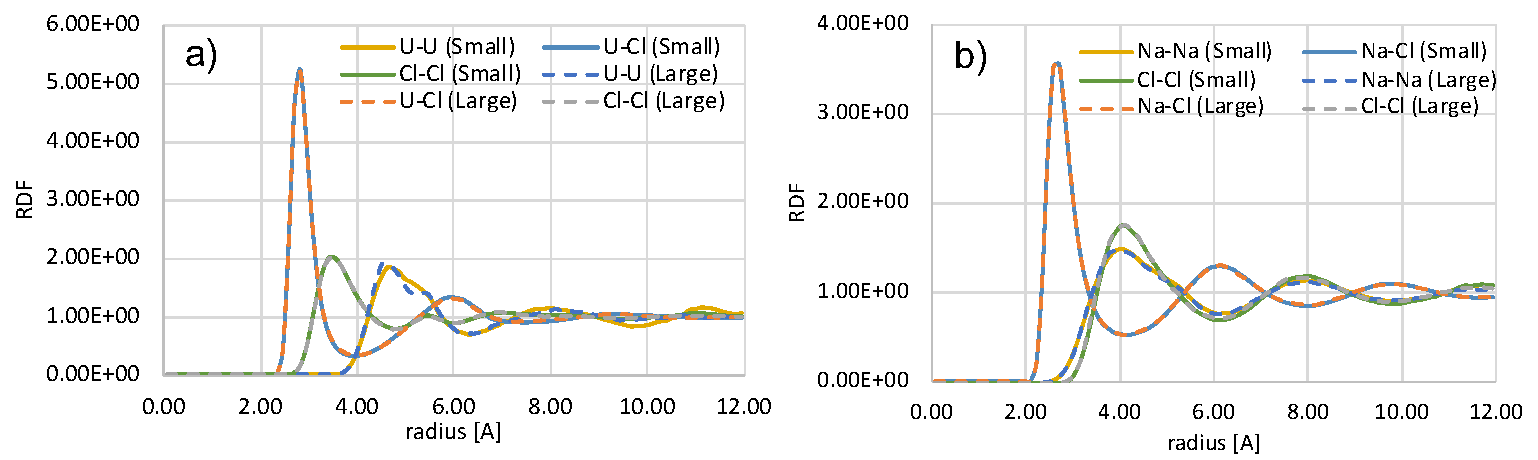
\includegraphics[width=0.45\textwidth]{FIG1_0.pdf}
\caption{The predicted radial distribution function for select cases compared to literature data. } 
\label{fig:radial}
\end{figure}


The AIMD simulations used the Projector Augmented Wave (PAW) method to describe the core electrons~\cite{}. For each element, the PAW potentials supplied with VASP for the PBE exchange-correlation potential were utilized. For Na, the version that only include the s electron(s)  in the valence shell was used for some of the simulations, while others us the version that also includes the semi-core p electrons. The difference between the two potentials will be discussed in Sec. \ref{sec:results}. Calculation of, for example, mixing energies in UCl$_3$-NaCl, can only be performed using a self-consistent data set (the same PAW potential), which is carefully enforced in the present study. The PAW potential for Cl also included p electrons and U included the outer s, p and f electrons in the valance shell. For some of the Van der Waals models, an alternate exchange-correlation potentials was utilized, namely the rPW86~\cite{}. Calculations were performed both with and without the Hubbard $U$ term, in order to capture the impact of accounting for strong electron correlation effects.
%than PBE, such as XX, were used.
%For the uranium 5f electrons, an additional Hubbard $U$  term was introduced in order to capture the effect of strong correlations. 
%Calculations were also performed with the standard exchange-correlation potential (no Hubbard $U$ model). 
The Lichtenstein approach~\cite{} was used for the Hubbard $U$  methodology and an approximate U value range of  3.0-4.5 eV was determined by using the constrained DFT linear-response method for crystalline UCl$_3$~\cite{}. The J value was set to 0.51 eV. These values are similar to those proposed for UO$_2$~\cite{}. After confirming that the values for UCl$_3$ were close to those for UO$_2$, the values for UO2 were adopted in the present study. Future work may consider further optimization of the Hubbard $U$  (and J) parameters, but the results and conclusions are not expected to change dramatically based on this choice, at least as long as the value is sufficiently large to ensure an insulating ground state. It should be noted that the effective U value depends on the coordination environment and consequently could differ between crystalline UCl$_3$ and molten salts. It could also be a function of time in the simulations as the environment may change. Future work may consider these questions in more detail, but it is beyond the scope of the present study. The effect of the Hubbard $U$  parameter for molten uranium chloride salts is the same as for crystalline UO$_2$; without the U parameter the salts are predicted to be metallic, which is contrary to the expected behavior, see Fig. \ref{fig:DOS}. Even though useful results may certainly be obtained while ignoring the strong correlations captured by the Hubbard $U$  parameter and accepting the resulting metallic character predicted for the salts, there are limitations to this approach. Uranium ions in its 3+ state have localized magnetic moments. Both ferro-magnetic and anti-ferromagnetic (AFM) orderings were investigated. In the context of molten salts, the AFM option is similar to a random distribution with a total magnetic moment in the supercell close to zero. The AFM ordering is slightly energetically preferred and sometimes results in better convergence behavior. However, the predicted properties are not influenced by the magnetic ordering in a measurable way.  Both the AFM and FM orderings are adopted in our simulations under the assumption that the thermodynamics and thermo-physical properties are only marginally affected by the choice.  


\begin{figure}[htb]
\centering
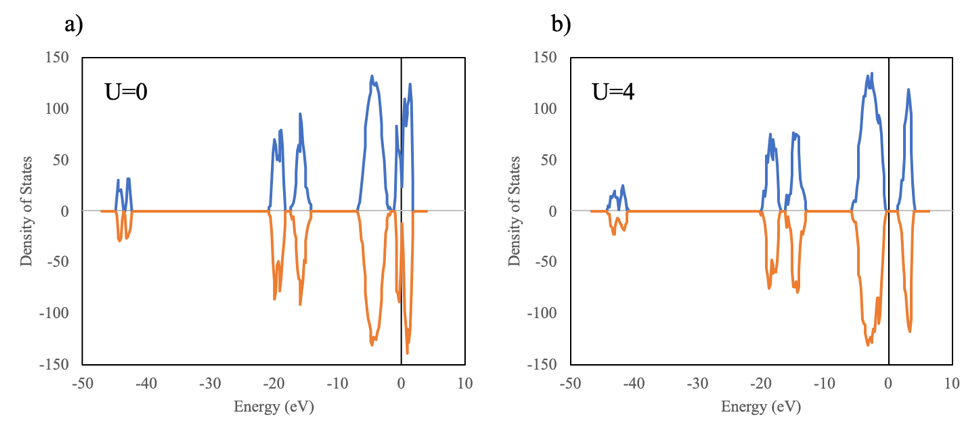
\includegraphics[width=\columnwidth]{figure2.png}
\caption{The spin-polarized predicted density of states for simulations of molten UCl$_3$ at 1250 K, a) not including and b) including a Hubbard $U$ model with U = 4 eV.} 
\label{fig:DOS}
\end{figure}


It is well-established in the literature that van der Waals or dispersion interactions are critical for reproducing the density of molten salts by DFT methods~\cite{}. Previous simulations have used both the DFT-D3 method~\cite{} and the Langreth \& Lundqvist~\cite{} methodologies for various molten chloride salts. Both methods are used in the present study and for the Langreth \& Lundqvist~\cite{}  methodology several exchange-correlation potentials were tested. In addition, the so-called dDsC method was also included in the set of Van der Waals models. The dDsC method is not implemented for f elements in the standard VASP version. In order to enable simulations the corresponding parameters were taken from Ref. \cite{}. 
%The supercells of molten salts were either created by melting the crystalline phases at high temperature for an expanded volume using an isochoric (NVT) thermostat with velocities scaled each time step or by XXX. The temperature used for melting the lattice was well above the experimental melting point. The temperature of the system was then slowly reduced to the simulation temperature of interest. These simulations were performed with lower accuracy settings than the equilibration and production runs described above. The melting procedure was only performed once for a specific temperature in the middle of the range of interest. Simulations for other temperatures were performed by decreasing or increasing the temperature from the initial molten reference structure created according to the procedure above.

The AIMD simulations for the molten salt supercells were performed using both isobaric conditions (NPT) and isochoric (NVT) conditions. The primary intent of the NPT simulations is to evaluate density, thermal expansion, heat capacity and mixing energy. The NVT simulations also allow calculation of the compressibility and species diffusion. Both the NPT and NVT ensemble simulations applied the Langevin thermostat in VASP.
For the NPT simulations, the temperature friction coefficients were set to 10 ps$^{-1}$ and the friction coefficient for the lattice degrees of freedom to 1 ps$^{-1}$. For the NVT simulations, the temperature friction coefficients were set to 2 ps$^{-1}$. The different  choice of friction coefficients for NPT and NVT does not impact the results and originate from the behavior of temperature fluctuations. The time step was set to 2 fs or lower for production runs at 1500 K or below, and 1 fs above this temperature. All simulations used pre-equilibrium runs that involve melting the lattice and ensuring convergence of the total energy for the temperature of interest. After pre-equilibration, production runs follow for at least (about) 20 ps, of which the final 15 ps were used to calculate properties. The 20 ps were either reached by performing consecutive runs or by combining results for independent simulations over a shorter period of time. Specifically, 5 independent runs were performed for 5 ps of which the final 4 ps were used to calculate properties. This is assumed to be yield approximately the same results as running a single simulation for 20 ps with the first 5 ps as preproduction time. Performing independent runs allow utilization of computational resources in a more efficient way. Some simulations used longer simulation times, in particular this applies to the simulations based on smaller supercells (up to 50 ps) and systems containing NaCl (up to 40 ps).  None of the results change significantly after the minimum simulation time stated above (20 ps with a production time of 15 ps).
%Pre-equilibrium runs were performed with a time-step of 5 fs. The pre-equilibration runs were performed for a minimum of 10 ps. Production runs were performed for a minimum of 10 ps for all systems, higher for NaCl and for the small supercells. The first 1-2 ps in the production runs were ignored in order to ensure that the results for the new time step was allowed to equilibrate. Obviously, longer runs would further improve statistics and would certainly be desired, but the convergence of thermo-physical and thermodynamic quantities was monitored and deemed to be sufficient for the present purpose.  
%which is rather large but motivated by the heavy uranium ions moving very slowly and the need to accumulate sufficient statistics to evaluate properties. 
%This time step still allows resolution of the dynamics of Na and Cl ions. Production runs were preceded by equilibration for at least 5 ps with data collected during a minimum of 15 ps. 

All properties were calculated by averaging over the production run (not including the equilibration or pre-production time). Densities were trivially obtained from the supercell volume and heat capacities from the slope of the total internal energy as function of temperature. Mixing enthalpies/energies were calculated from the potential energy of the mixed salt with pure NaCl and UCl$_3$ at the same temperature as reference. The compressibility is calculated as the negative of the inverse equilibrium volume multiplied by the derivative of the volume as a function of pressure. The diffusivities are calculated from the mean square displacements through the Einstein relation. 

\section{Results}
\label{sec:results}
\subsection{Benchmark of methodology for molten NaCl}
Figure \ref{fig:NaCldensity} plots the predicted density of molten NaCl as function of temperature for the DFT-D3, dDsC and Langreth \& Lundqvist dispersion models as well as simulations without any dispersion interaction. A correlation derived from experimental data is also shown~\cite{}. All simulations reproduce the temperature dependence of the density obtained from experiments. However, as expected, only the simulations that account for dispersion interactions are within 10\% of the experimental density correlation. The best agreement is obtained for the Langreth \& Lundqvist and dDsC dispersion models, which are within 5\% or less of the experimental correlation across an extended temperature range. The calculated (Langreth \& Lundqvist  and dDsC) and experimental correlation for the density as function of temperature are listed in Table~\ref{table:densityetc}.


\begin{figure}[htb]
\centering
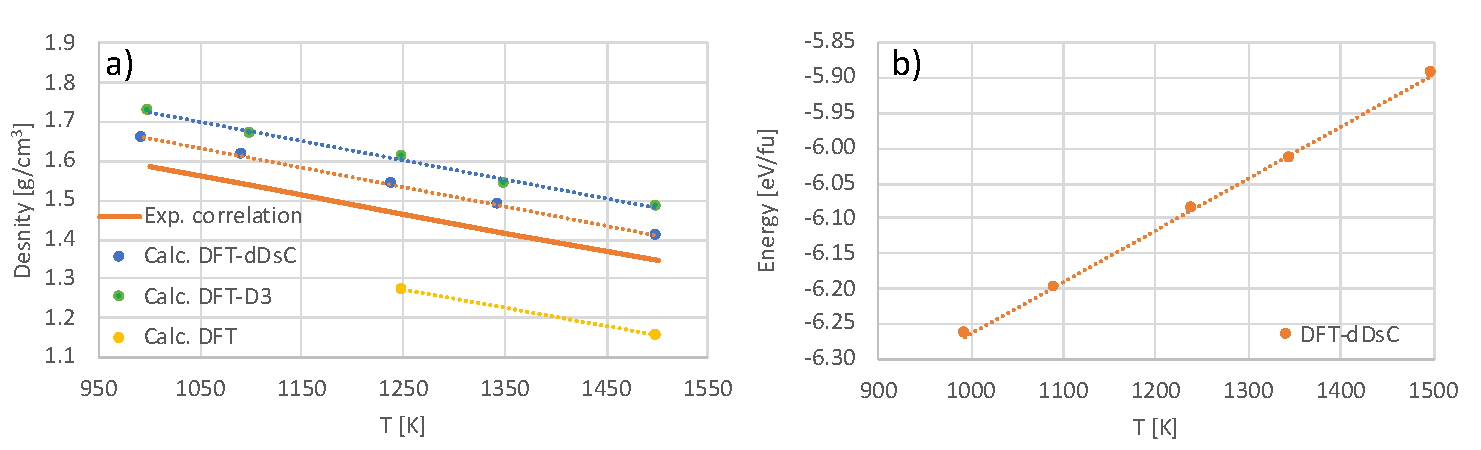
\includegraphics[width=0.45\textwidth]{FIG2.pdf}
\caption{Density of NaCl predicted with three different models for dispersion forces and one without. Experimental data is represented by the correlation plotted as an orange line~\cite{}. Note that the temperature range of the experimental correlation and some data points extend beyond the boiling point of NaCl, which is solely for illustrative purposes. The lines shown are least-squares fits to the calculated data points.} 
\label{fig:NaCldensity}
\end{figure}


\begin{table*}[hb!]
\centering
\begin{tabular}{lccc}
\hline
\hline
& Density (g/cm$^3$)	&Heat capacity (J/mol/K) &Compressibility ()\\
\hline
NaCl Calculated (D3)	& & &\\
NaCl Calculated (dDsC)	& & &\\
NaCl Calculated (Langreth \& Lundqvist)	& & &\\
NaCl Experiment	& & &\\
UCl$_3$ Calculated (Langreth \& Lundqvist) & & & \\	
UCl$_3$ Calculated (dDsC) & & & \\	
UCl3 Experiment	& & & \\
\hline
\hline
\end{tabular}
\caption{Calculated and experimental correlations for density, heat capacity and compressibility as function of temperature for NaCl and UCl$_3$. The first quantity is a linear function of temperature, while the latter two are constants.}
\label{table:NaCldensityetc}
\end{table*}
 
Fig. \ref{fig:NaClheatc} plots the potential energy per formula unit of molten NaCl as function of temperature. The derivative equals the heat capacity of NaCl, which is also tabulated in Table \ref{table:NaCldensityetc} together with an experimental reference valu~\cite{}e. The simulation results indicate a constant heat capacity. The good agreement between simulations and experiments for the heat capacity further emphasizes the accuracy of the AIMD simulations.  

\begin{figure}[htb]
\centering
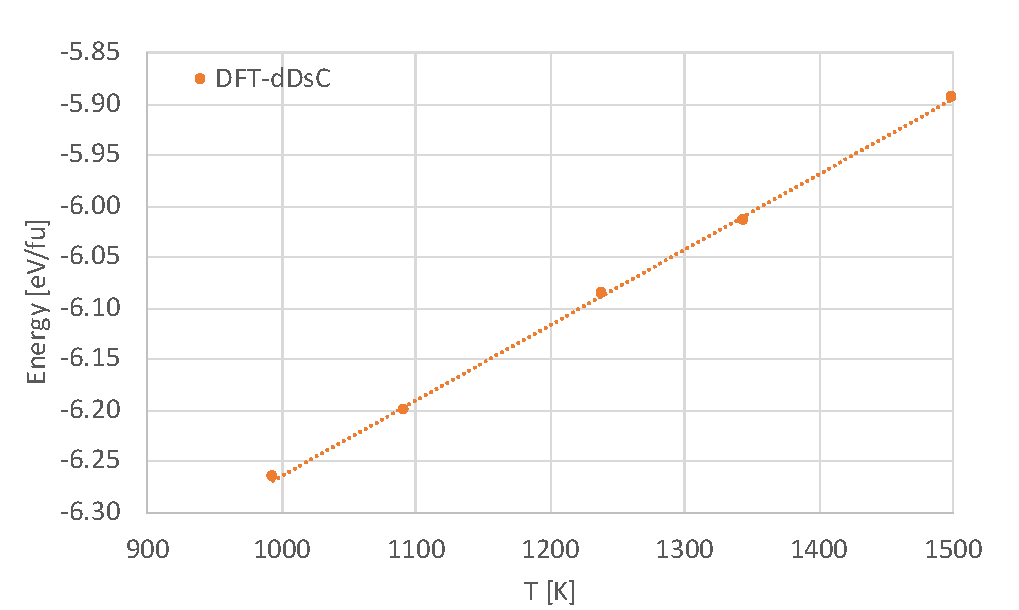
\includegraphics[width=0.45\textwidth]{FIG3.pdf}
\caption{Calculated potential energy of NaCl as function of temperature. The line is a least-squares fit to data points and the slope represents the heat capacity.} 
\label{fig:NaClheatc}
\end{figure}

The results in Figs. \ref{fig:NaCldensity} and \ref{fig:NaClheatc} refers to simulations based on the large supercells. Fig. \ref{fig:NaClsize} compares these results with those obtained from the supercells. Density and heat capacity are both accurately represented by the smaller supercells, at least below 1750 K, which supports the accuracy of the results with respect to the supercell size. It also suggests that at least for NaCl, the larger supercell is not required to achieve converged results for density and heat capacity at moderate temperature (below 1750 K). Some deviation is observed for the highest temperature, which may be related to approaching the boiling temperature. 


\begin{figure}[htb]
\centering
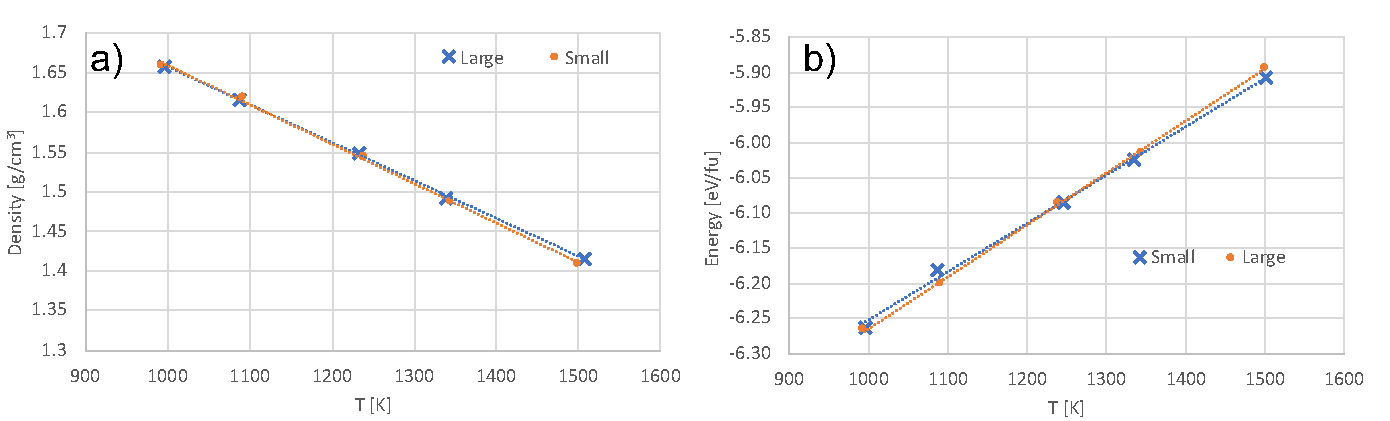
\includegraphics[width=0.45\textwidth]{FIG3b.pdf}
\caption{a) Calculated density and b) potential energy of NaCl as function of temperature for the large and small supercells. The line is a least-squares fit to data points and the slope represents the heat capacity.} 
\label{fig:NaClsize}
\end{figure}


The NVE simulations also allow calculation of the compressibility and diffusivity of each species. These results are also summarized in Table \ref{table:NaCldensityetc} (compressibility) and Table \ref{table:NaCldiffusivityetc}.

 \begin{table*}[hb!]
\centering
\begin{tabular}{lccc}
\hline
\hline
&Na	(m$^2$/s)&Cl (m$^2$/s)&U (m$^2$/s)\\
\hline
Diffusivity NaCl & & &\\
Diffusivity UCl$_3$	& & &\\
Diffusivity NaCl-UCl$_3$ & & &\\
\hline
\hline
\end{tabular}
\caption{Calculated diffusivities for each species in NaCl, UCl$_3$ and  NaCl-UCl$_3$.}
\label{table:NaCldiffusivityetc}
\end{table*}

\subsection{AIMD simulations for UCl$_3$}
Following the benchmark for NaCl, the next step is to apply the most accurate methodologies (Langreth \& Lundqvist and dDsC) to UCl$_3$ with a few spot checks using the other Van der Waals models as well. 

Figure \ref{fig:UCl3density} plots the predicted density for UCl$_3$ as function of temperature for the Langreth \& Lundquist and dDsC dispersion models, with a few spot checks for other Van der Waals models (DFT-D3), and compares the results to two literature correlations derived from experiments~\cite{}. The two experimental correlations are surprisingly different and cannot both be valid, except in a narrow temperature range. Recently reported experimental data~\cite{} confirm the model due to XX et al.~\cite{}. The most recent experimental data set agrees well with the simulation data, with both the Langreth \& Lundqvist and dDsC model predicting values within a few per cent of the experimental data. The temperature dependence is predicted to be linear across the full temperature range investigated. The Langreth \& Lundqvist methodology is sensitive to the choice of exchange -correlation potential. The optimal choice proved excellent agreement with experiments, while other choices may lead to significant underestimation of the density despite performing very well for the NaCl benchmark system. Note that only a single point was calculated for the DFT-D3 model, but that indicates essentially the same behavior as the dDsC model.  Compared to the Desytniak correlation~\cite{},  the predicted temperature dependence of the density is slightly different. It agrees better with the more recent experimental data points~\cite{XX}. The effect of including the Hubbard $U$  model is to decrease the density (increase the volume) compared to the reference case, which follows the expected behavior extrapolated from uranium compounds such as UO$_2$. The densities in Figure \ref{fig:UCl3density} were fitted to linear correlations and summarized in Table \ref{table:NaCldensityetc}.


\begin{figure}[htb]
\centering
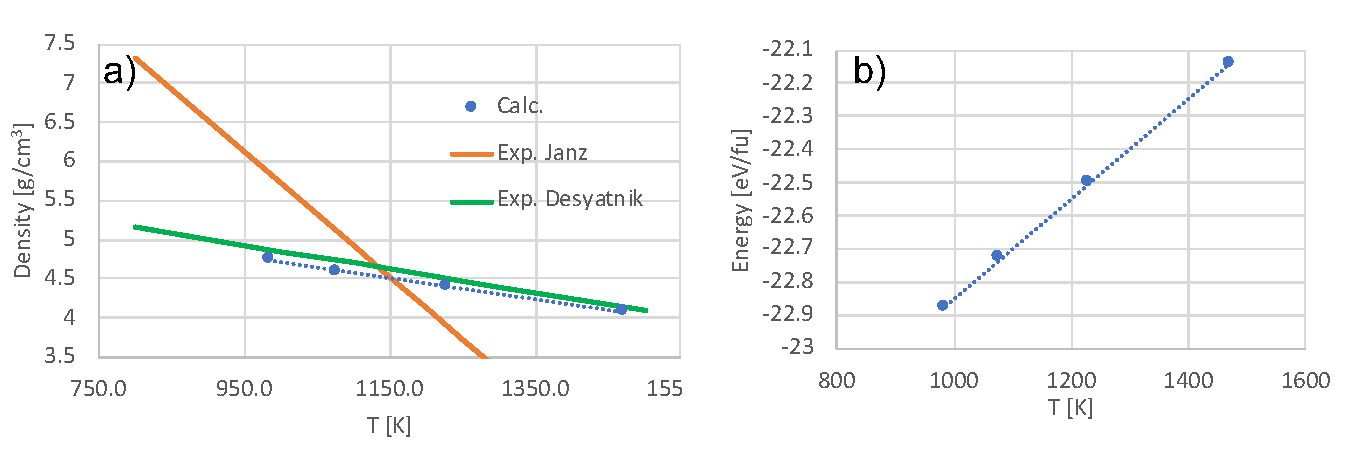
\includegraphics[width=0.45\textwidth]{FIG4.pdf}
\caption{Density of UCl$_3$ predicted with different models for the dispersion forces and one without. Experimental data is represented by the correlations plotted as blue lines and XX.~\cite{}. The lines are least-squares fits to the calculated data points, the equations of which are summarized in Table \ref{table:NaCldensityetc.}} 
\label{fig:UCl3density}
\end{figure}

 
Figure \ref{fig:fig:UCl3heat} plots the potential energy as function of temperature, from which the heat capacity can be derived by calculating the slope. We have not been able to identify experimental data on UCl$_3$, but our results compare very well with the value derived from the current CALPHAD UCl$_3$ database (see Table~\ref{table:NaCldiffusivityetc})~\cite{}.

\begin{figure}[htb]
\centering
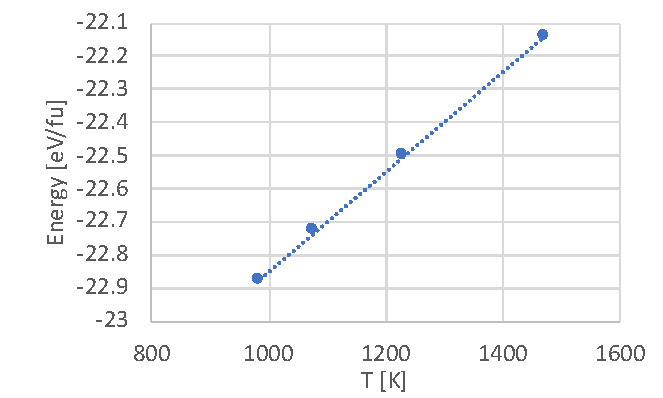
\includegraphics[width=0.45\textwidth]{FIG5.pdf}
\caption{Calculated potential energy of UCl$_3$ as function of temperature. The line is a least-squares fit to data points and the slope represents the heat capacity.} 
\label{fig:UCl3heat}
\end{figure}


The results discussed so far for UCl$_3$ were generated with the large supercells. These results are compared to those derived from the smaller supercells in Fig. \ref{fig:UCl3size}, which, similar to NaCl, exhibits good agreement with each other. This provides confidence in the convergence of the current results.

\begin{figure}[htb]
\centering
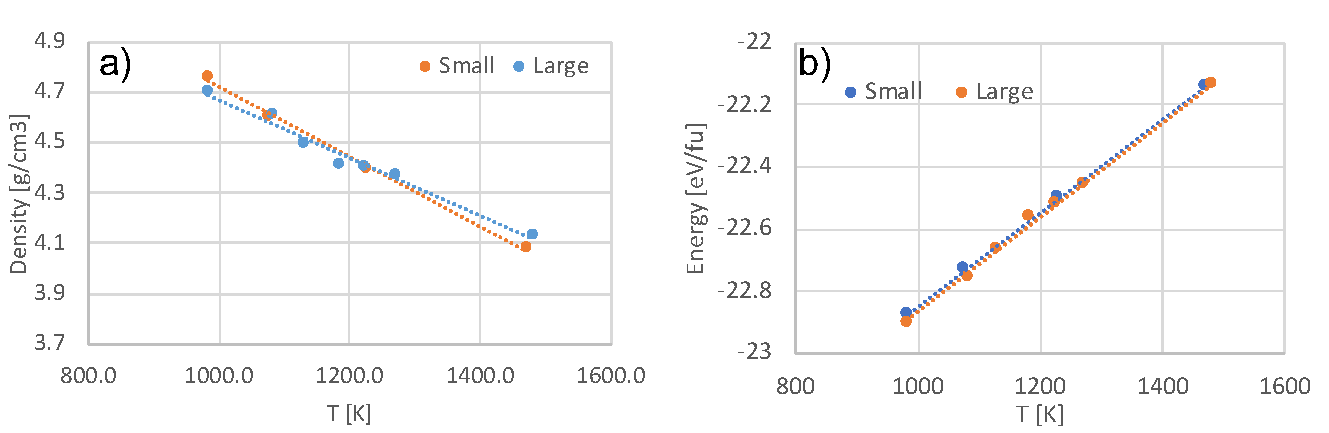
\includegraphics[width=0.45\textwidth]{FIG4b.pdf}
\caption{Calculated density and potential energy of UCl$_3$ as function of temperature for the large and small supercells. The line is a least-squares fit to data points and the slope represents the heat capacity.} 
\label{fig:UCl3size}
\end{figure}

As for NaCl, The NVE simulations also allow calculation of the compressibility and diffusivity of each species. These results are  summarized in Table \ref{table:NaCldensityetc} (compressibility) and Table \ref{table:NaCldiffusivityetc}.
 
\subsection{AIMD simulations for NaCl-UCl$_3$}
The density of NaCl-UCl$_3$ mixtures were calculated for the Langreth \& Lundqvist and dDsC dispersion models at 1200K and 1250K, as shown in Figure \ref{fig:NaClUCl3}. This figure also shows experimental results from Desyatnik et al.~\cite{} and lines corresponding to an ideal mixture of the end members. The insets highlight the deviation form ideal solution behavior. The simulation data points are within a few per cent of the experimental data and close to the ideal mixture. Both simulations and experiments suggest a negative deviation from an ideal solution (lower density than predicted by an ideal solution behavior). Although there is some spread in the data points that we ascribe to sampling uncertainties, there is a minimum about 3\% below the ideal solution density close to the eutectic composition. The experimental data also shows a negative deviation, including a minumum close to the eutectic composition.  

\begin{figure}[htb]
\centering
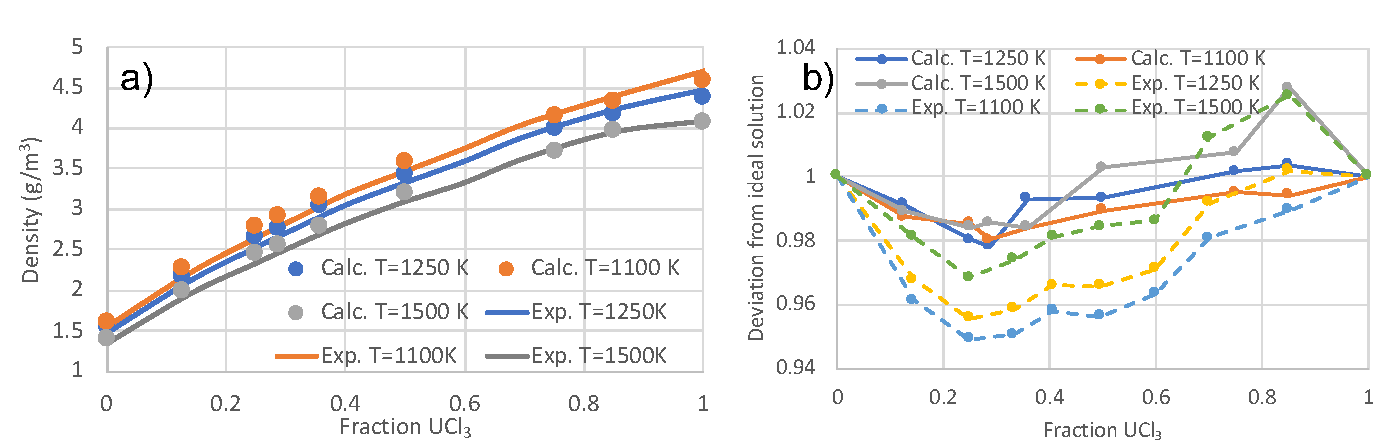
\includegraphics[width=0.45\textwidth]{FIG6.pdf}
\caption{a) Density of NaCl-UCl$_3$ mixtures as obtained from simulations and experimental data~\cite{} at 1250K. The lines represent an ideal solution with the calculated and experimental NaCl and UCl$_3$ densities as end points. The deviation form ideal solution behavior is highlighted in the inset. b) Same as a) but performed using a different simulation methodology at 1200 K. Results for both the large and small supercells are shown.} 
\label{fig:NaClUCl3}
\end{figure}

The total energies of the NaCl-UCl$_3$ mixtures at 1250 K and 1200 K are plotted in Figure \ref{fig:NaClUCl3e}, with the NaCl and UCl$_3$ end members as reference points, which confirms the close to ideal mixture behavior already observed for the densities. As for the density, a minimum is observed close to the eutectic composition. 

Although the simulations were run long enough to sample the configuration space, it is possible that the initial distribution of Na and U ions have some impact on the results, especially for the large supercells.  In order to test this possibility, a few of the Na And Cl atoms in the previous simulations were swapped and the simulations were re-run. In particular we target the compositions that seemed to deviate from the overall trend somewhat. Indeed, the new simulations provided slightly different results in closer agreement with the trends already discussed. For the large cells, this is an inherent uncertainty of the simulation apporach.

\begin{figure}[htb]
\centering
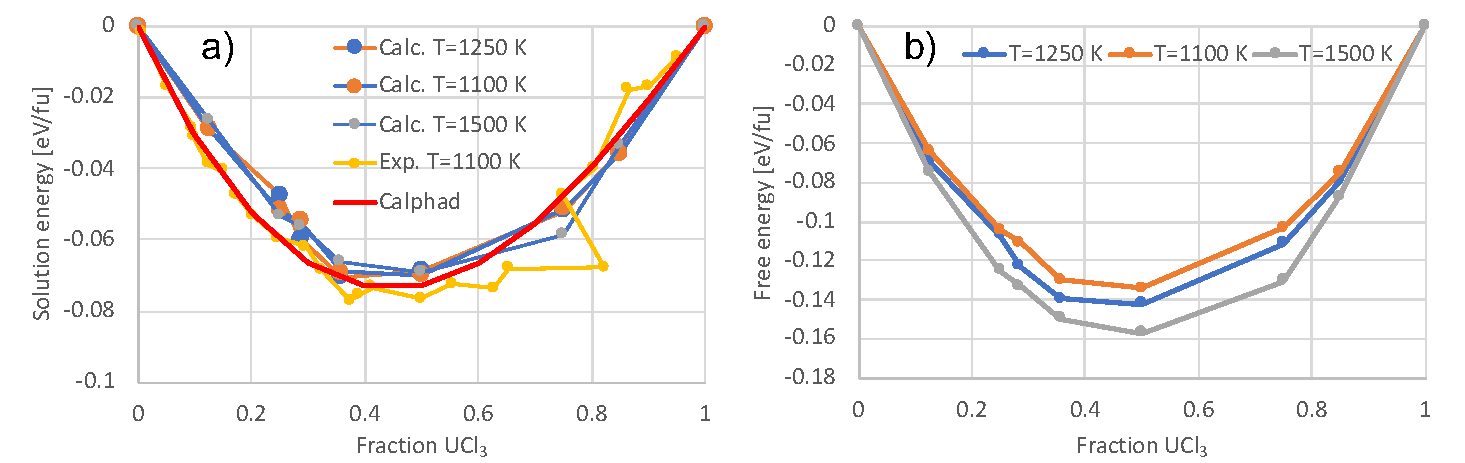
\includegraphics[width=0.45\textwidth]{FIG7.pdf}
\caption{a) Mixing energies for NaCl-UCl$_3$ mixtures at 1250 K. Pure NaCl and UCl$_3$ are used as references. The solid black line represents the zero-mixing energy for the ideal solution. b) Same as a) but performed using a different simulation methodology at 1200 K. Results for both the large and small supercells are shown.} 
\label{fig:NaClUCl3e}
\end{figure}

The comparison between large and small supercells for the density and mixing energy are also shown in Figs. \ref{fig:NaClUCl3} and \ref{fig:NaClUCl3e}. Unlike the cases of NaCl and UCl$_3$, the NaCl-UCl$_3$ mixture exhibit some deviation between the supercells for one of the compositions, although the trends are still the same. 

\section{Discussion}
\label{sec:discussion}

\section{Conclusions}
\label{sec:conclusions}


\section{Acknowledgments}



\bibliographystyle{elsarticle-num-names}
\bibliography{beelerbib}

\end{document}
